% Lecture Template for ME3023 -  Measurements in Mechanical Systems - Tennessee Technological University
% Spring 2020 - Summer 2020 - Fall 2020 - Spring 2021 - Summer 2021 - Fall 2023
% Tristan Hill, May 07, 2020 - June 12, 2020 - July 08, 2020 - Novemeber 02, 2020 - March 28, 2021 - May 25, 2021 - August 21, 2022 - September 02, 2023 - September 09, 2023

% Fall 2023 - condensing and streamlining lectures by combining topics into a single PDF under the module name
%			  this will simplify file and link management as well as make lectures easier to use in class
%			- added image/ to clean directory and reduce redundancy, specific to module for now  

% Module Name: - Time Varying Circuits
% Topic 1 - The Dynamics of Circuits
% Topic 2 - First Order Systems
% Topic 3 - ---


\documentclass[fleqn]{beamer} % for presentation (has nav buttons at bottom)

\usepackage{/home/tntech.edu/thill/courses/measurements/lectures/measurements_lectures}
%\usepackage{/home/thill/courses/measurements/lectures/measurements_lectures}
%\usepackage{/mnt/c/Users/thill/Documents/courses/measurements/lectures/measurements_lectures}

\author{ME3023 - Measurements in Mechanical Systems} % original formatting from Mike Renfro, September 21, 2004

\newcommand{\MNUM}{4\hspace{2mm}} % module number 
\newcommand{\moduletitle}{Time Varying Circuits}

\newcommand{\sectionItitle}{The Dynamics of Circuits}
\newcommand{\sectionIItitle}{First Order Systems}
\newcommand{\sectionIIItitle}{---}

\newcommand{\sectionIsubsectionItitle}{Review Electrical Quantities}
\newcommand{\sectionIsubsectionIItitle}{Resistance and Impedance}
\newcommand{\sectionIsubsectionIIItitle}{Capacitance and Inductance}
\newcommand{\sectionIsubsectionIVtitle}{Example: RC Circuit}

\newcommand{\sectionIIsubsectionItitle}{General System Model}
\newcommand{\sectionIIsubsectionIItitle}{Mechanical-Electrical Analogies}
\newcommand{\sectionIIsubsectionIIItitle}{Example: RC Circuit}
\newcommand{\sectionIIsubsectionIVtitle}{Activity: Bulb Thermometer}

\newcommand{\sectionIIIsubsectionItitle}{---}
\newcommand{\sectionIIIsubsectionIItitle}{---}
\newcommand{\sectionIIIsubsectionIIItitle}{---}
\newcommand{\sectionIIIsubsectionIVtitle}{---}

 \newcommand{\btVFill}{\vskip0pt plus 1filll}

% custom box
\newsavebox{\mybox}

\title{Lecture Module - \moduletitle}

\date{Mechanical Engineering\vspc Tennessee Technological University}

\begin{document}

	\lstset{language=MATLAB,basicstyle=\ttfamily\small,showstringspaces=false}

	\frame{\titlepage \center\begin{framed}\Large \textbf{Module \MNUM - \moduletitle}\end{framed} \vspace{5mm}}

	% Module Outline
	\begin{frame} 
		\large \textbf{Module \MNUM - \moduletitle} \vspace{3mm}\\

		\begin{itemize}
			\item Topic 1 - \hyperlink{sectionI}{\sectionItitle} \vspc % section I
			\item Topic 2 - \hyperlink{sectionII}{\sectionIItitle} \vspc % section II
			\item Topic 3 - \hyperlink{sectionIII}{\sectionIIItitle} \vspc % section III
		\end{itemize}

	\end{frame}

	% section I
	\section{\sectionItitle}\label{sectionI}

		% section I Outline
		\begin{frame} 
			\large \textbf{Topic 1 - \sectionItitle} \vspace{3mm}\\

			\begin{itemize}
				\item \hyperlink{sectionIsubsectionI}{\sectionIsubsectionItitle} \vspc %  section I subsection I
				\item \hyperlink{sectionIsubsectionII}{\sectionIsubsectionIItitle} \vspc % section I subsection II
				\item \hyperlink{sectionIsubsectionIII}{\sectionIsubsectionIIItitle} \vspc % section I subsection III
				\item \hyperlink{sectionIsubsectionIV}{\sectionIsubsectionIVtitle} \vspc % section I subsection IV
			\end{itemize}
		\end{frame}
		
		% section I subsection I 
		\subsection{\sectionIsubsectionItitle}\label{sectionIsubsectionI}

			\begin{frame}
				\frametitle{\sectionIsubsectionItitle}

				\small
				\begin{itemize}

					\begin{multicols}{2}
					\item {\BL Charge} - the physical property of matter that causes it to experience a force when placed in an electromagnetic field.
					
					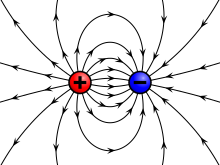
\includegraphics[scale=.5]{images/charges_plus_minus.png}
					\end{multicols}
					
					\item {\PR Voltage} - the difference in electric potential between two points ... can be caused by electric charge, by electric current through a magnetic field, by time-varying magnetic fields, or some combination of these three.
					
					\item {\RD Current} - the rate of flow of electric charge past a point or region. An electric current is said to exist when there is a net flow of electric charge through a region.

				\end{itemize}
							

			\end{frame}

			\begin{frame}
				\frametitle{\sectionIsubsectionItitle}

						\bigskip
						\begin{itemize}


						\item {\BL Resistance} - a measure of a components opposition to the flow of electric current. The inverse quantity is electrical conductance, and is the ease with which an electric current passes.  
						
						
						\item {\PR Capacitance} - the ratio of the change in electric charge of a system to the corresponding change in its electric potential (voltage).
						
						\item {\RD Inductance} - the tendency of an electrical conductor to oppose a change in the electric current flowing through it. The flow of electric current creates a magnetic field around the conductor. The field strength depends on the magnitude of the current, and follows any changes in current.

					\end{itemize}
							
	
		

			\end{frame}

		% section I subsection II
		\subsection{\sectionIsubsectionIItitle}\label{sectionIsubsectionII}

			\begin{frame}
				\frametitle{\sectionIsubsectionIItitle}

					\small
					\begin{multicols}{2}

						... electrical {\PN impedance} is the measure of the opposition that a circuit presents to a current when a voltage is applied. \vspc
						
						The term impedance was coined by Oliver Heaviside in July 1886. Arthur Kennelly was the first to represent impedance with complex numbers in 1893.
						
						\[ Z=\frac{V}{I}=\frac{|V|}{|I|}e^{j\left(\phi_V-\phi_I \right)} \] \vspace{2mm}
						\[ R=\frac{V}{I} \]

					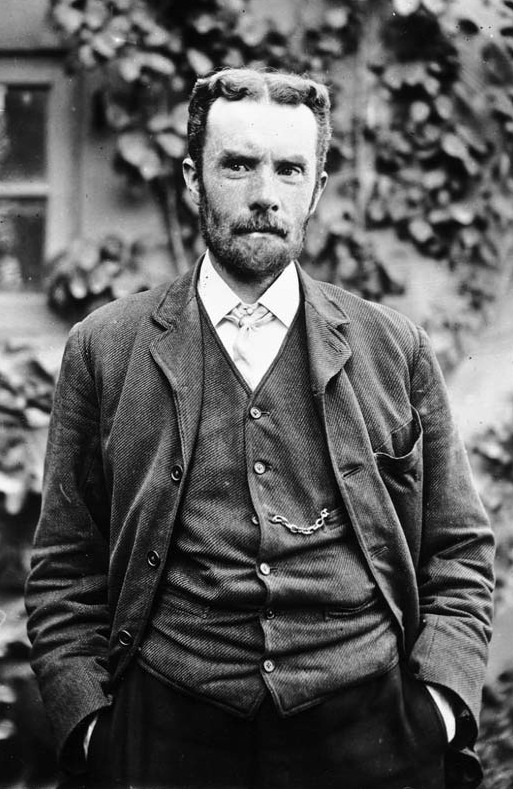
\includegraphics[scale=.2]{images/Oliver_Heaviside.jpg}\\
					{\tiny \href{https://en.wikipedia.org/wiki/Oliver_Heaviside}{Wikipedia}}

					\end{multicols}	

		
			\end{frame}

			\begin{frame}
				\frametitle{\sectionIsubsectionIItitle}

					In addition to {\PR resistance} as seen in DC circuits, {\PN impedance} in AC circuits includes the effects of the induction of voltages in conductors by the magnetic fields (inductance), and the electrostatic storage of charge induced by voltages between conductors (capacitance). The impedance caused by these two effects is collectively referred to as reactance and forms the imaginary part of complex impedance whereas resistance forms the real part. 

{\tiny \href{https://en.wikipedia.org/wiki/Electrical_impedance}{Wikipedia}}

	

			\end{frame}


			\begin{frame}

						\bigskip  
			


			\end{frame}

			\begin{frame}




		
			\end{frame}





		% section I subsection III
		\subsection{\sectionIsubsectionIIItitle}\label{sectionIsubsectionIII}
			\begin{frame} 
				\frametitle{\sectionIsubsectionIIItitle}

				\bigskip

					In many DC applications the transient, or dynamic, behavior of the circuit must be considered. This may be counter-intuitive. \vspc
	
		{\PR Capacitance} - the ratio of the change in electric charge of a system to the corresponding change in its electric potential (voltage). \vspc

	\begin{fleqn}
		\[i_C(t)=C\frac{dv_C\left(t\right)}{dt} \] \vspace{2mm}
		\[v_C=\frac{1}{C}\int\limits_{t_1}^{t_2}i_C(t)dt \]
	\end{fleqn}







			\end{frame}	

			\begin{frame} 
				\frametitle{\sectionIsubsectionIIItitle}

	{\RD Inductance} - the tendency of an electrical conductor to oppose a change in the electric current flowing through it. The flow of electric current creates a magnetic field around the conductor. The field strength depends on the magnitude of the current, and follows any changes in current. \vspc
	
	\begin{fleqn}
	\[v_L(t)=L\frac{d}{dt}i_L(t)=L\frac{di_L}{dt} \] 	
	\[i_L(t)=\frac{1}{L}\int\limits_{t_1}^{t_2}v_L\left(t\right)dt \]
	\end{fleqn}



				
			\end{frame}	

		% section I subsection IV
		\subsection{\sectionIsubsectionIVtitle}\label{sectionIsubsectionIV}	

			\begin{frame}
				\frametitle{\sectionIsubsectionIVtitle}

				\bigskip


	The basic RC circuit is a simple but important example that I assume you saw in your circuits course. This circuit demonstrates a fundamental concept and has several practical uses in mechanical measurements. \vspc
	
	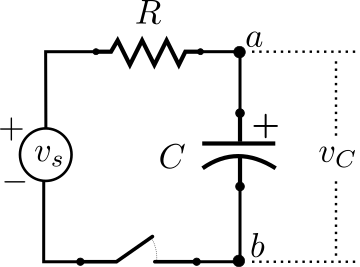
\includegraphics[scale=0.5]{images/rc_circuit.png}


		
				
			\end{frame}

			\begin{frame}
				\frametitle{\sectionIsubsectionIVtitle}

\bigskip


			\end{frame}

	
	% Section II
	\section{\sectionIItitle}\label{sectionII}

		% section II Outline
		\begin{frame}
			\large \textbf{Topic 2 - \sectionIItitle} \vspace{3mm}\\

			\begin{itemize}
				\item \hyperlink{sectionIIsubsectionI}{\sectionIIsubsectionItitle} \vspc %  section II subsection I
				\item \hyperlink{sectionIIsubsectionII}{\sectionIIsubsectionIItitle} \vspc % section II subsection II
				\item \hyperlink{sectionIIsubsectionIII}{\sectionIIsubsectionIIItitle} \vspc % section II subsection III
				\item \hyperlink{sectionIIsubsectionIV}{\sectionIIsubsectionIVtitle} \vspc % section II subsection IV
			\end{itemize}

		\end{frame}

		% section II subsection I
		\subsection{\sectionIIsubsectionItitle}\label{sectionIIsubsectionI}

			\begin{frame}[label=sectionIIsubsectionI]
				\frametitle{\sectionIIsubsectionItitle}

				The behavior of a circuit is dependent on time, and many common circuits can be represented by a {\it linear ordinary differential equation} which can be written in the following standard form. 

\[ a_n\frac{d^nx}{dt^n}+a_{n-1}\frac{d^{n-1}x}{dt^{n-1}}+...+a_2\frac{d^2x}{dt^2}+a_1\frac{dx}{dt}+a_0x=f(t) \] 
\vspace{0mm}
	



			\end{frame}

		    \begin{frame}[label=sectionIIsubsectionI]
				\frametitle{\sectionIIsubsectionItitle}





			\end{frame}	

		% section II subsection II
		\subsection{\sectionIIsubsectionIItitle}\label{sectionIIsubsectionII}

			\begin{frame}
				\frametitle{\sectionIIsubsectionIItitle}


				Many mechanical systems are also time dependent, or {\it dynamic} and a mechanical-electrical analog is often draw between the two.

\renewcommand{\arraystretch}{1.5}
\begin{tabular}{ccc}
\underline{Zero Order}&\underline{First Order}&\underline{Second Order}\\
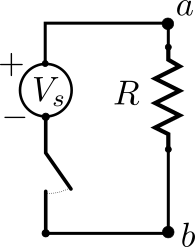
\includegraphics[scale=0.25]{images/r_circuit.png}&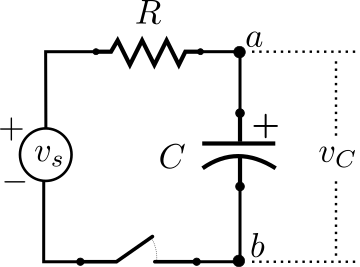
\includegraphics[scale=0.25]{images/rc_circuit.png}&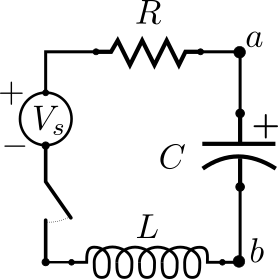
\includegraphics[scale=0.25]{images/rlc_circuit.png}\\
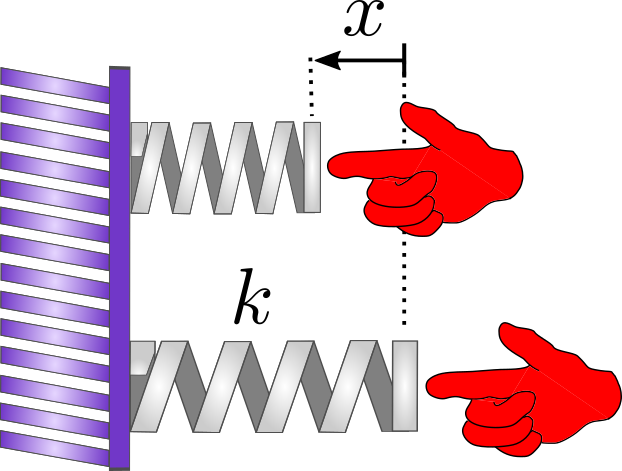
\includegraphics[scale=0.15]{images/hand_spring.png}&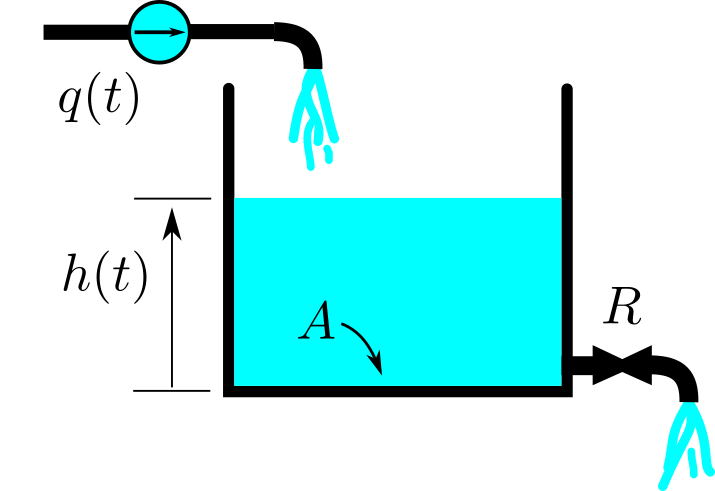
\includegraphics[scale=0.15]{images/water_tank.png}&\hspace{5mm}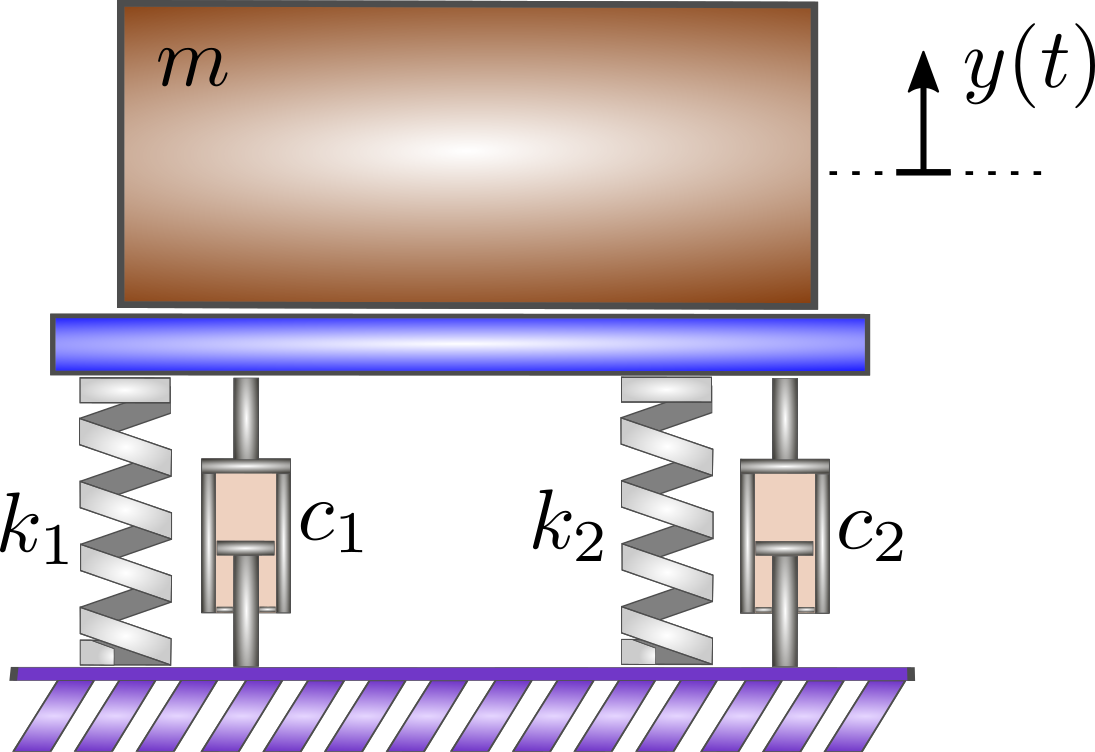
\includegraphics[scale=0.10]{images/mass_spring_damper.png}\\
\end{tabular}

This concept {\it was} used for analysis and simulation. 
				


			\end{frame}

		% section II subsection III
		\subsection{\sectionIIsubsectionIIItitle}\label{sectionIIsubsectionIII}

			\begin{frame}
				\frametitle{\sectionIIsubsectionIIItitle}

				The RC circuit is a first order system. The response to a step input $v_s$ is exponential which is described a single parameter the time constant $\tau$. 
\vspc

\begin{multicols}{2}
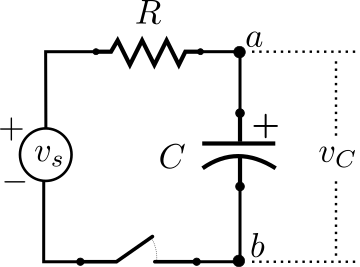
\includegraphics[scale=0.5]{images/rc_circuit.png} 	
	
First Order Model
\begin{fleqn}
\[ RC\dot{v}_C+v_C=v_S \]
\end{fleqn}

Response Equation
\begin{fleqn}
\[v_C\left(t\right)=v_s\left(1-e^{-\frac{t}{RC}}\right) \]
\end{fleqn}

\end{multicols}


			\end{frame}		

			\begin{frame}
				\frametitle{\sectionIIsubsectionIIItitle}

				\bigskip

				\begin{multicols}{2}

\renewcommand{\arraystretch}{1.5}
\begin{tabular}{|c|c|} \hline
$time (s)$&$response (V)$\\ \hline
&\\ \hline
&\\ \hline
&\\ \hline
&\\ \hline
\end{tabular}

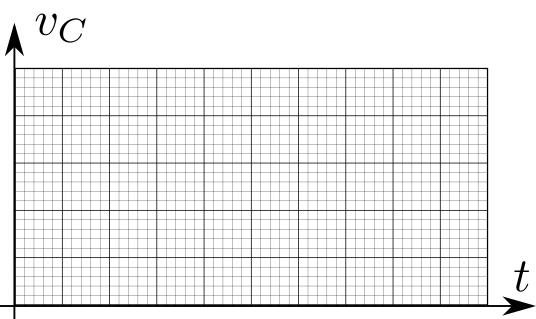
\includegraphics[scale=0.5]{images/voltage_versus_time.png} 	
\end{multicols}



			\end{frame}

			\begin{frame}
				\frametitle{\sectionIIsubsectionIIItitle}

			\end{frame}

			\begin{frame}
			\frametitle{\sectionIIsubsectionIIItitle}





			\end{frame}

		% section II subsection IV 
		\subsection{\sectionIIsubsectionIVtitle}\label{sectionIIsubsectionIV}

			\begin{frame}
				\frametitle{\sectionIIsubsectionIVtitle}


{\scriptsize \underline{Activity:} This should be completed by each student as an individual. You are encouraged to discuss with your peers. }

Consider the bulb thermometer shown which can be modeled as a first order system.  Write the system model and the expected reponse.

\[ \frac{dE}{dt}=\dot{Q}\hspace{15mm} \frac{dE}{dt}=mc_v\frac{T(t)}{dt} \hspace{15mm}\dot{Q}=hA_s\Delta T \]
\[ \]

\begin{multicols}{2}

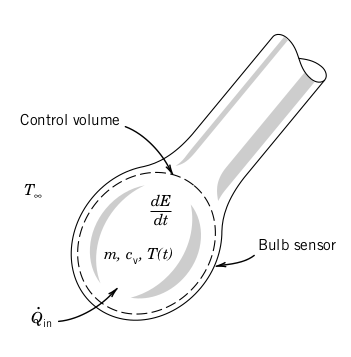
\includegraphics[scale=.35]{images/bulb_thermometer.png}

First Order Model:
\begin{fleqn}
\[ mc_v\frac{T(t)}{dt}+hA_sT(t)=hA_sT_\infty \] 
\end{fleqn}

Response Equation:
\begin{fleqn}
\[ T(t)=T_\infty+\left[ T\left(0\right)-T_\infty \right]e^{-\frac{t}{\tau}} \] 
\end{fleqn}


\end{multicols}


			\end{frame}

			\begin{frame}
				\frametitle{\sectionIIsubsectionIVtitle}

				{\scriptsize \underline{Activity:} Fill out the table below and sketch a graph to represent the data. }

\begin{multicols}{2}

\renewcommand{\arraystretch}{1.5}
\begin{tabular}{|c|c|} \hline
$time (s)$&$response (^\circ C)$\\ \hline
0&\\ \hline
$1\tau$&\\ \hline
$2\tau$&\\ \hline
$3\tau$&\\ \hline
$4\tau$&\\ \hline
\end{tabular}

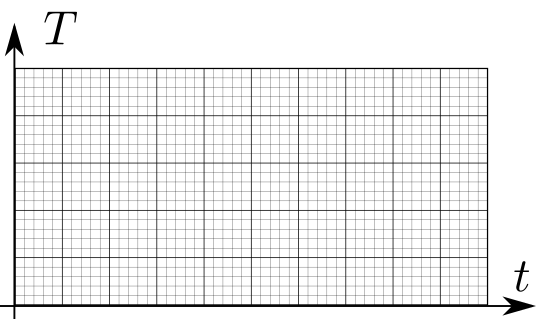
\includegraphics[scale=0.5]{images/temp_versus_time.png} 	
\end{multicols}



			\end{frame}

			\begin{frame}

			{\scriptsize \underline{Activity:} Answer the following questions. }\\{ \tiny (hint: Think about the {\it general system model}.)}\\


What is the time constant of the bulb thermometer system? 

\vspace{5mm}
\begin{fleqn}
\[ \tau= \]
\end{fleqn}
\vspace{5mm}\\What is the static sensitivity? What are the units?
\vspace{5mm}
\begin{fleqn}
\[ K= \]
\end{fleqn}
\vspace{8mm}


			\end{frame}


		
	% Section III
	\section{\sectionIIItitle}\label{sectionIII}

		% section III Outline
		\begin{frame}
			\large \textbf{Topic 3 - \sectionIIItitle} \vspace{3mm}\\

			\begin{itemize}
				\item \hyperlink{sectionIIIsubsectionI}{\sectionIIIsubsectionItitle} \vspc %  section III subsection I
				\item \hyperlink{sectionIIIsubsectionII}{\sectionIIIsubsectionIItitle} \vspc % section III subsection II
				\item \hyperlink{sectionIIIsubsectionIII}{\sectionIIIsubsectionIIItitle} \vspc % section III subsection III
				\item \hyperlink{sectionIIIsubsectionIV}{\sectionIIIsubsectionIVtitle} \vspc % section III subsection IV
			\end{itemize}

		\end{frame}

		% section III subsection I
		\subsection{\sectionIIIsubsectionItitle}\label{sectionIIIsubsectionI}

			\begin{frame}
				\frametitle{\sectionIIIsubsectionItitle}

			
				
			\end{frame}

			\begin{frame}
				\frametitle{\sectionIIIsubsectionItitle}
		
			\end{frame}

		% section III subsection II
		\subsection{\sectionIIIsubsectionIItitle}\label{sectionIIIsubsectionII}	

			\begin{frame}
				\frametitle{\sectionIIIsubsectionIItitle}

	

			\end{frame}

		% section III subsection III
		\subsection{\sectionIIIsubsectionIItitle}\label{sectionIIIsubsectionIII}

			\begin{frame}
				\frametitle{\sectionIIIsubsectionIIItitle}

		

			\end{frame}

			\begin{frame}
				\frametitle{\sectionIIIsubsectionIIItitle}



			\end{frame}

		% section III subsection IV
		\subsection{\sectionIIIsubsectionIVtitle}\label{sectionIIIsubsectionIV}	

			\begin{frame}
				\frametitle{\sectionIIIsubsectionIVtitle}

			


			\end{frame}

			\begin{frame}
				\frametitle{\sectionIIIsubsectionIVtitle}
				


			\end{frame}

\end{document}





